\documentclass[border={-3 4 -4 -5}]{standalone}

\usepackage{physics}
\newcommand{\mcD}{\mathcal{D}}

\usepackage{graphicx}
\graphicspath{{../}}

\usepackage{tikz}

\begin{document}
\small
\begin{tikzpicture}
\begin{scope}[shift={(0,0)}]
% Mean level spacing ratio{{{
\node (listdensityplotr) at (0,0) 
  {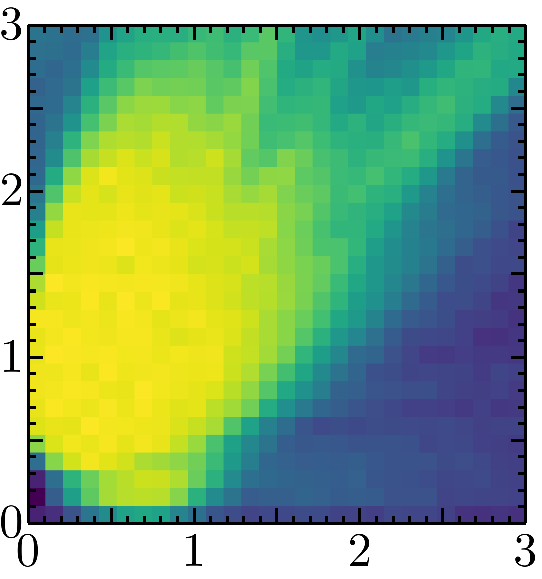
\includegraphics[width=0.325\textwidth]{mean_level_spacing_ratio_ising_L_16_hx_1_even_parity.pdf}};% mapa de color
\node (barlegend) at (listdensityplotr.north) [anchor=south, inner sep=-10pt]  {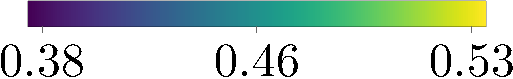
\includegraphics[width=0.27\textwidth]{mean_level_spacing_ratio_ising_bar_legend.pdf}};% barra de leyenda

%Etiquetas 
\node[rotate=90] () at (listdensityplotr.west) [] {$J/h_x$};
\node (labelr) at (barlegend.north) [anchor=south, inner sep=8pt] {$\ev{\tilde r}$};
\node () at (listdensityplotr.south) [anchor=north, inner sep=-5pt] {$h_z/h_x$};
%}}}

% Averaged purity{{{
\node (chaometer) at ([xshift=-10pt,yshift=-0.2pt]listdensityplotr.east) [anchor=west] 
  {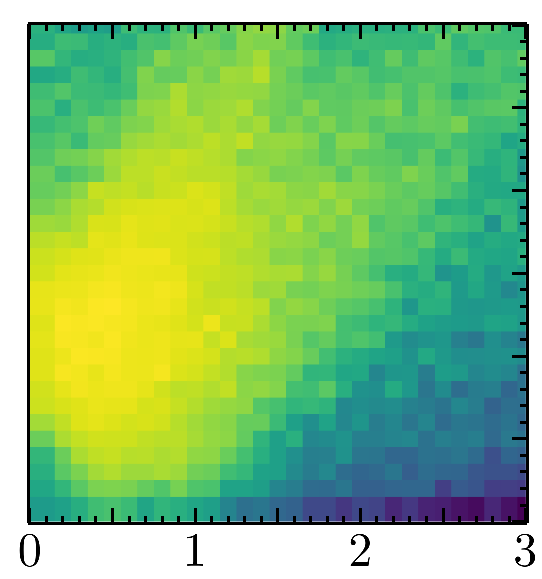
\includegraphics[height=0.345\textwidth]{chaometer_purity_ising_L_7_hx_1.pdf}};%mapa de color
\node (legendChaometer) at (chaometer.north) [anchor=south, inner sep=-10pt]  
  {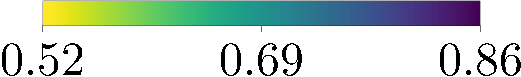
\includegraphics[width=0.27\textwidth]{chaometer_purity_ising_bar_legend.pdf}};% bara para leyenda

\node (labelChaometer) at (legendChaometer.north) [anchor=south, inner sep=9pt] {$\overline{\mathcal{P}}$};
\node () at (chaometer.south) [anchor=north, inner sep=-5pt] {$h_z/h_x$};
%}}}

% Averaged Choi purity{{{
\node (choi) at ([xshift=-6.5pt,yshift=-2pt]chaometer.east) [anchor=west] 
  {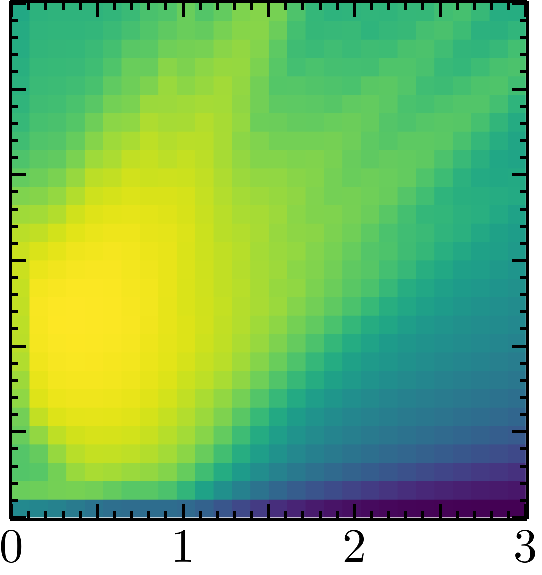
\includegraphics[height=0.33\textwidth]{temporal_avg_haar_avg_choi_purity_ising_L_7_hx_1.pdf}};% mapa de color
\node (legendChoi) at (choi.north) [anchor=south, inner sep=-2pt]  
  {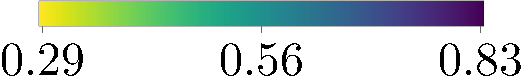
\includegraphics[width=0.27\textwidth]{temporal_avg_haar_avg_choi_purity_ising_bar_legend.pdf}};% barra de leyenda
%
\node (labelchoi) at (legendChoi.north) [anchor=south, inner sep=2pt] {$\ev{\Tr[\mcD(t)^2]}_{\mathrm{Haar}, T}$};
\node () at (choi.south) [anchor=north, inner sep=-5pt] {$h_z/h_x$};
%}}}

% Letras{{{
\node (a) at ([xshift=-1.56cm, yshift=0.1cm]labelr.west) {(a)};
\node (b) at ([xshift=3.8cm, yshift=0pt]a.east) {(b)};
\node (c) at ([xshift=3.5cm, yshift=0pt]b.east) {(c)};
%}}}

\draw[red, dashed, line width=0.9pt, opacity=0.7] (-1.76,-0.5) -- (1.85,-0.5);
\draw[red, dashed, line width=0.9pt, opacity=0.7] (2.05,-0.5) -- (5.65,-0.5);
\draw[red, dashed, line width=0.9pt, opacity=0.7] (5.85,-0.49) -- (9.45,-0.49);

\end{scope}
\end{tikzpicture}
\end{document}